\section{Auswertung}
\subsection{Ermitteln des Brechungsindex einer Glasprobe}
	Nach der in Abschnitt \ref{sec:shimadzu} beschriebenen Messung des spektralen Transmissions- und Reflexionsvermögens einer vorgegebenen (Quarz-)Glasprobe im Wellenlängenbereich von $\lambda = 250\dots800\ \unit{nm}$ ergeben sich die in Abbildung \ref{fig:R_T_glas} dargestellten Spektren.
	\begin{figure}[ht]
		\centering
		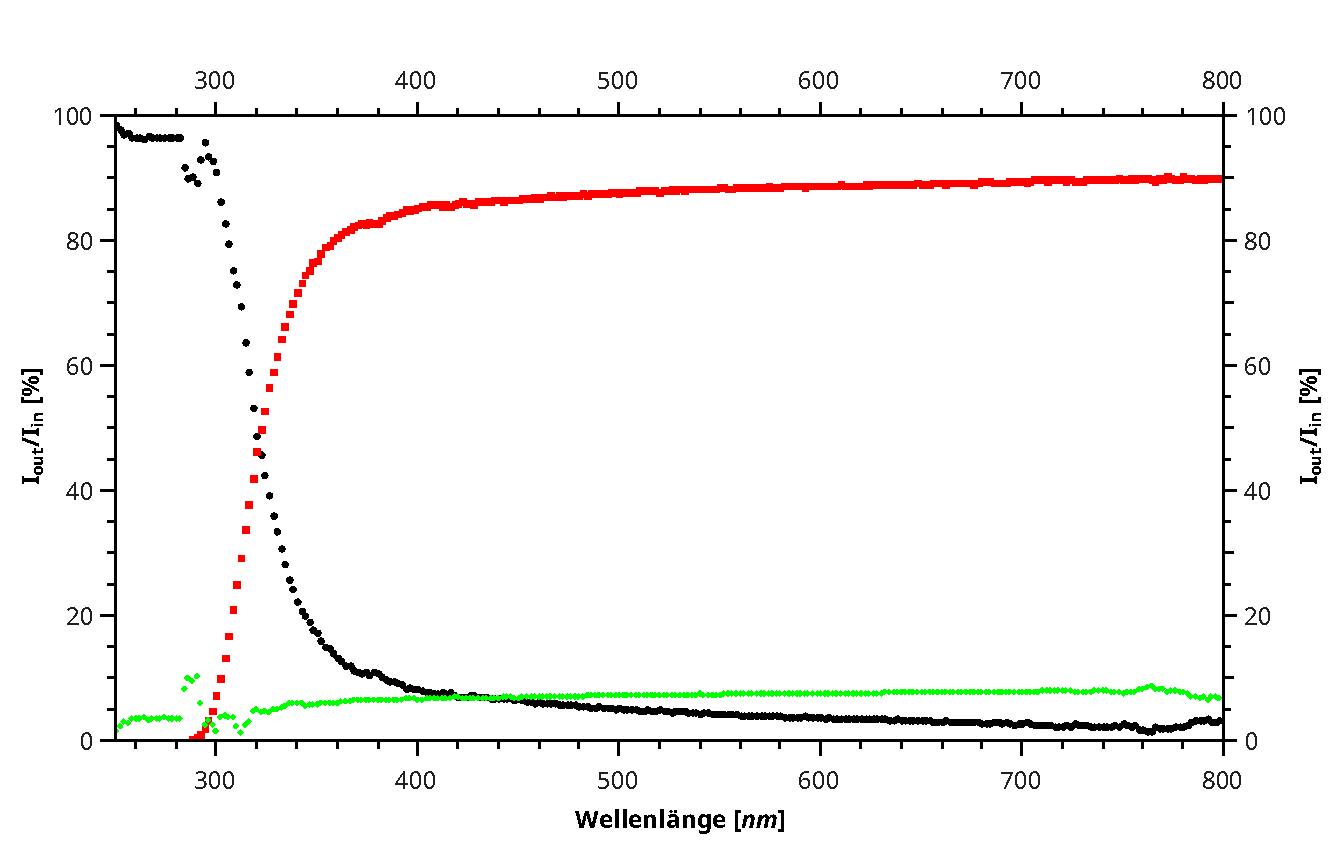
\includegraphics[width=\linewidth]{pic/R_T_glas.pdf}
		\caption{Spektrales Transmissions- (rot), Reflexions- (grün) und Absorptionsvermögen (schwarz) einer Glasprobe. Aufgetragen ist das Verhältnis der Intensität des Probestrahles $I_{out}$ zu der des Referenzstrahles $I_{in}$ in Abhänigkeit der Wellenlänge des Strahles $\lambda$.}
		\label{fig:R_T_glas}
	\end{figure}
	Dabei wurde angenommen, dass das Absorptionsvermögen durch $A = 1 - R - T$ gegeben ist. Man sieht deutlich, dass das Glas wie ein Kantenfilter wirkt, welcher elektromagnetische Wellen unterhalb einer Wellenlänge von $\unit[300]{nm}$ absorbiert. Im sichtbaren Bereich von etwa 400 bis $\unit[800]{nm}$ ist das Glas hauptsächlich transparent, da das Transmissionsvermögen etwa $\unit[90]{\%}$ beträgt.\\
	Mit Hilfe der Formeln (\ref{eq:n_T}) und (\ref{eq:n_R}) kann aus dem Spektrum der wellenlängenabhängige Brechungsindex bestimmt werden. Abbildung \ref{fig:n_glas} zeigt den Verlauf für die Berechnung aus dem Transmissions- und dem Reflexionsvermögen.
	\begin{figure} [ht]
				\centering
				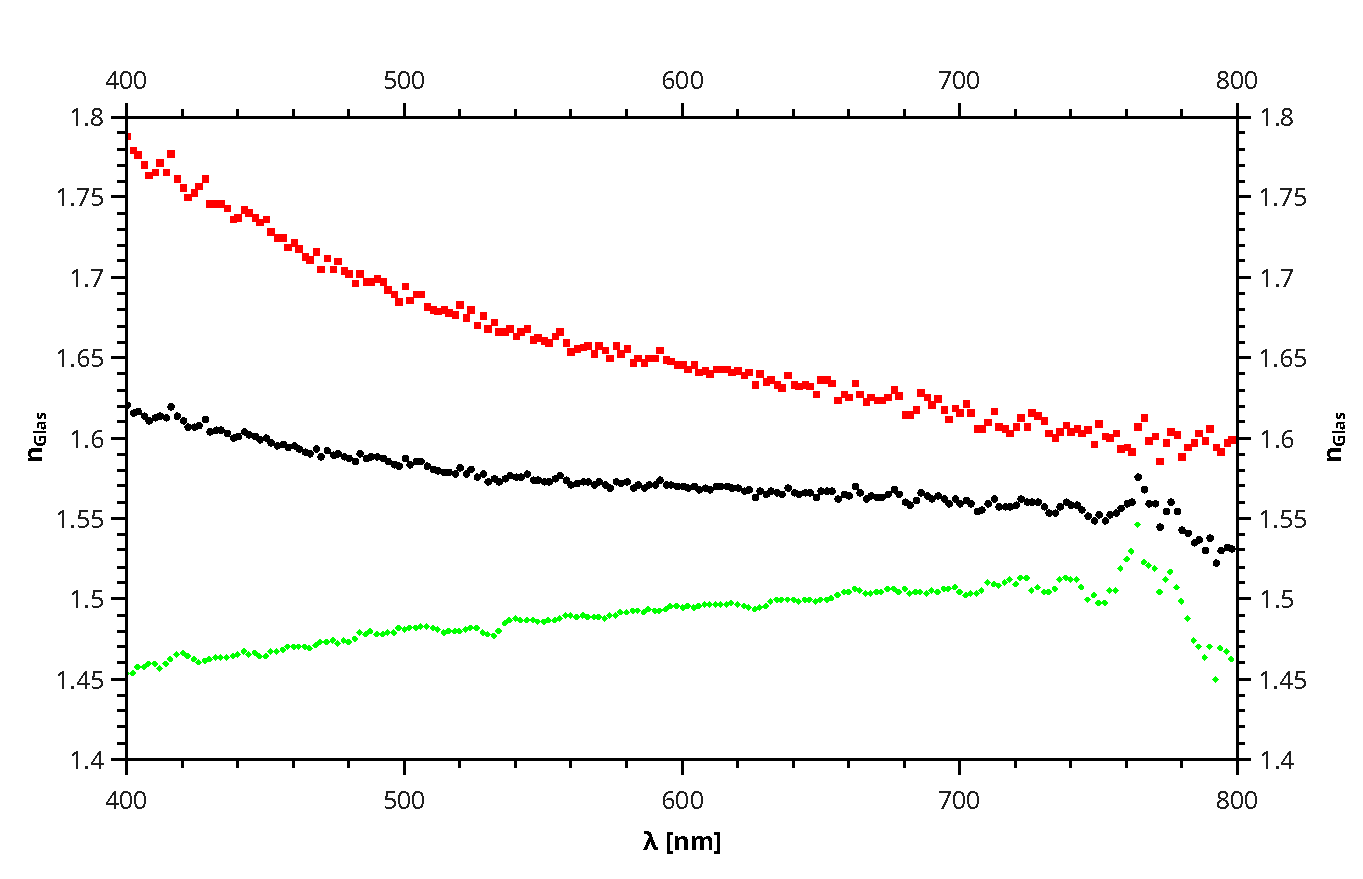
\includegraphics[width=\linewidth]{pic/n_glas.pdf}
				\caption{Wellenlängenabhängiger Brechungsindex. Dieser wurde aus dem Transmissionsvermögen (rot), dem Reflexionsvermögen (grün) bestimmt und anschließend gemittelt (schwarz).}
				\label{fig:n_glas}
	\end{figure} 
	Beide Berechnungen sollten theoretisch zu einem identischen Ergebnis führen, was offensichtlich nicht der Fall ist. Ein möglicher Grund dafür ist die Tatsache, dass Absorption im Medium stattfindet und somit die Relation $1 = T_{ges} + R_{ges}$, die in der Herleitung aus Abschnitt (\ref{sec:fresnel}) verwendet wurde, nicht gültig ist. Da die Absorption allerdings schwach im Vergleich zur Transmission ist, ist die obige Herleitung eine akzeptable Näherung. Mittelt man beide errechnete Werte, erhält man den erwarteten Verlauf, dass der Brechungsindex im sichtbaren Bereich für große Wellenlängen immer weiter abnimmt. Dieser Effekt wird \textit{Dispersion} genannt und er erklärt die spektrale Aufspaltung von Licht, die beispielsweise an einem Glasprisma auftritt. Mittelt man über den gesamten sichtbaren Wellenlängenbereich erhält man einen mittleren Brechungsindex für den vorliegenden Glasfilter von:
	\begin{equation}
		\bar{n} = 1,57 \pm 0,02.
	\end{equation}
	Hierbei steht die Fehlerangabe für die Standardabweichung der aufgenommenen Messpunkte um den Mittelwert.\\
	Für Wellenlängen unterhalb  von $\unit[400]{nm}$ ist es nicht sinnvoll den Brechungsindex mit der oben angegebenen Methode zu berechnen, da Absorptionseffekte immer signifikanter werden. Um dies noch besser zu berücksichtigen müsste man den Brechungsindex als komplexe Größe auffassen, d.h. $n \rightarrow N := n(1 + \kappa) \in \mathbb{C}$.
	
\subsection{Transmissions- und Reflexionsvermögen verschiedener Filter}
	Im Folgenden sollen die Ergebnisse der in Abschnitt \ref{sec:shimadzu} beschriebenen Messungen des spektralen Transmissions- und Reflexionsvermögens diverser Proben qualitativ diskutiert werden.
    \subsubsection{Farbfilter}
        In Abschnitt \ref{sec:fluoromax} werden zuerst bunte Glasplatten untersucht. Das sind Platten aus Quarzglas, in deren Struktur zusätzlich zum Quarz andere Teilchen eingebracht wurde. In den Abbildungen \ref{exp:farbT} und \ref{exp:farbR} sind die Ergebnisse der Relfexions- und Transmissionsmessung zu sehen.
        \begin{figure}
            \subfigure[Farfilter Transmission\label{exp:farbT}]{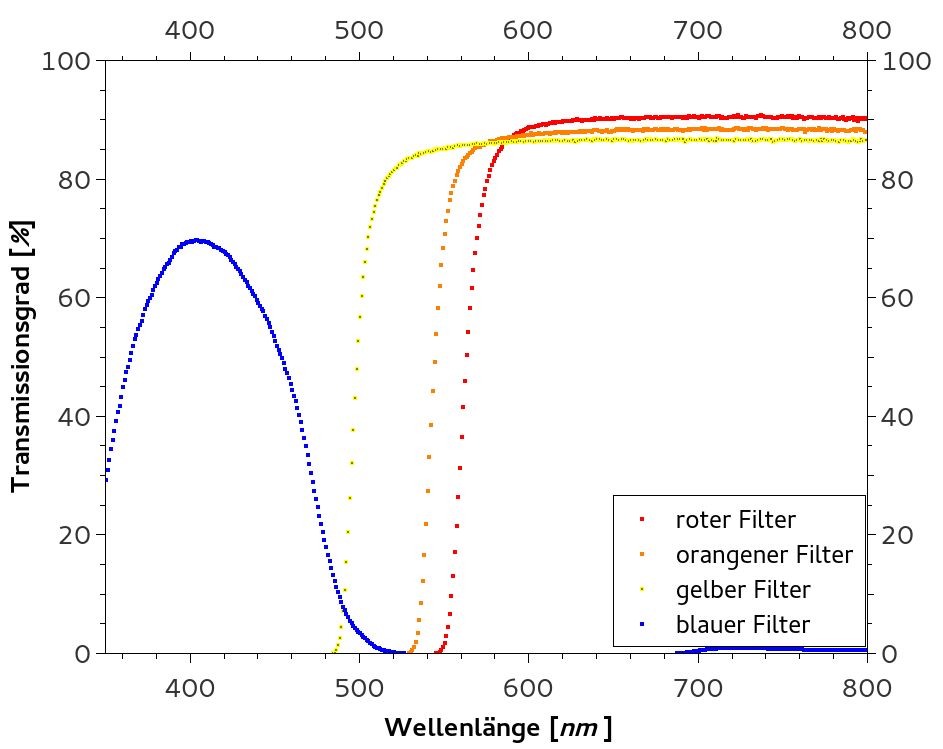
\includegraphics[scale=.25]{pic/TFarbfilter.png}}
            \subfigure[Farbfilter Reflexion\label{exp:farbR}]{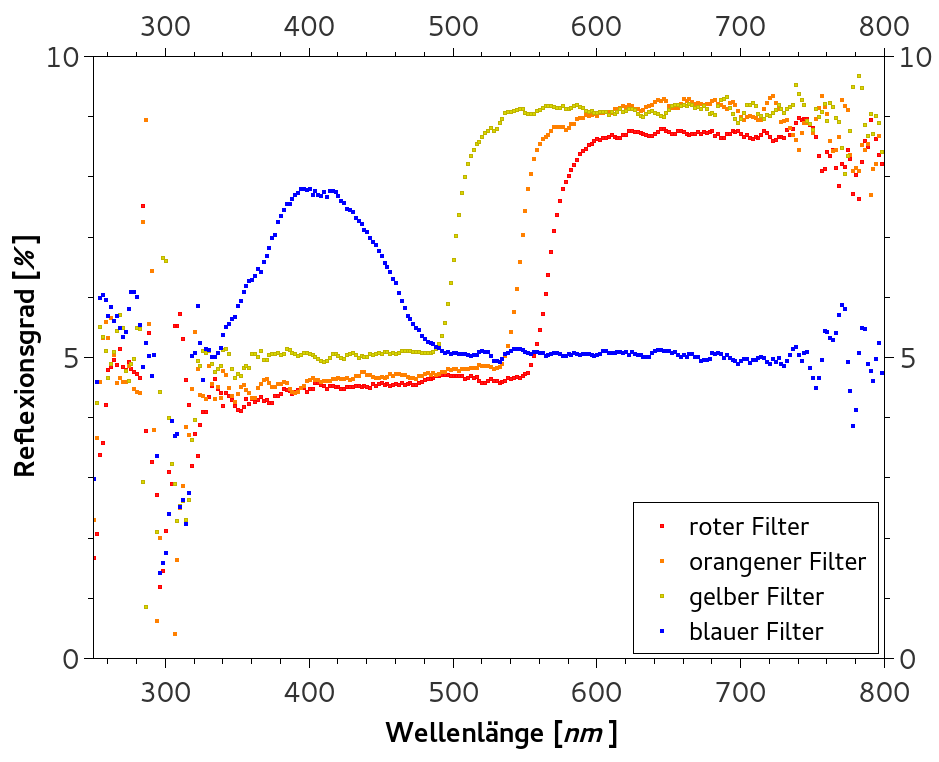
\includegraphics[scale=.25]{pic/RFarbfilter.png}}
            \caption{Reflexions- und Transmissionsgrade von farbigen Gläsern}
            \label{exp:farb}
        \end{figure}
        Die Filter $rot$, $orange$ und $gelb$ nennt man Kantenfilter. Das liegt an ihrer charakteristischen Kante. Der $blaue$ Filter wird Gauß-Filter genannt. Dies liegt an seinem charakteristischem Messkurvenverlauf, welcher einer typischen Glockenkurve ähnelt. Die Reflexion der Maxima bei allen Farbfiltern ist deutlich geringer als ihr Transmissionsvermögen in den gleichen Intervallgrenzen. Dieses Verhalten ist erwartungsgemäß, da die Filter alle durchsichtig sind und somit mehr Licht durch sie hindurch gelassen als von ihnen reflektiert wird.\\
        In Abbildung \ref{exp:farbR} kann man Fluktuationen um $285\unit{nm}$ erkennen, welche zum einen durch den Lampenwechsel, zum anderen auch durch den Wechsel der Messbereiche der Detektoren zustande kommt.
        Für die Kantenfilter gilt weiterhin, dass der Absorptionsgrad links der Kante nahezu $100\unit{\%}$ beträgt, was gerade der jeweiligen Komplementärfarbe entspricht. Rechts der Kante findet kaum Absorption statt.
    \subsubsection{Metallinterferenzfilter}
        Als nächstes wurde wird ein Filter untersucht, welcher auf der einen Seite grün, auf der anderen Seite metallisch glänzte. Untersucht wurde die Transmission in Abhängigkeit von verschiedenen Winkeln und der Wellenlänge. Genaue Winkel wurden dazu nicht notiert. Weiterhin wurde die Reflexion der Metallschicht sowie der grünen Schicht untersucht. (vgl. Abbildung \ref{exp:MetInt})
        \begin{figure}
            \subfigure[Transmission eines Metallinterferenzfilters in Abhängigkeit verschiedener Winkel\label{exp:TMetInt}]{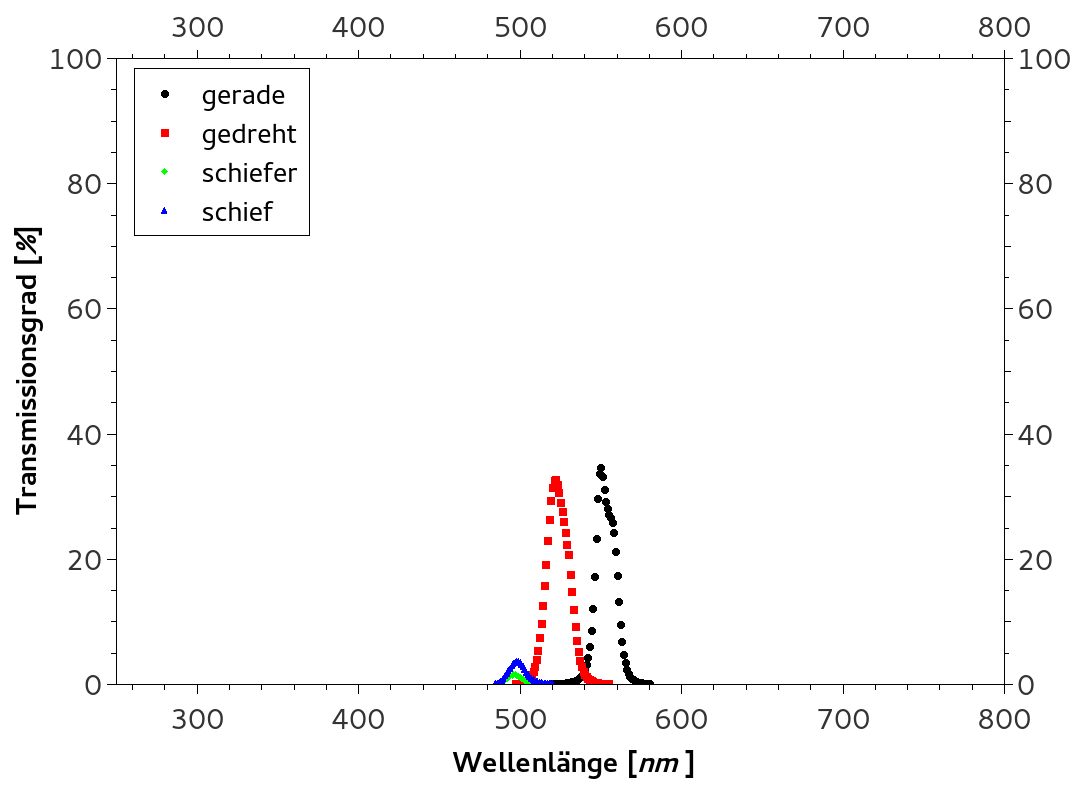
\includegraphics[scale=.22]{pic/TmetIntFilt.png}}
            \subfigure[Reflexion eines Metallinterferenzfilters in Abhängigkeit von der Seite\label{exp:RMetInt}]{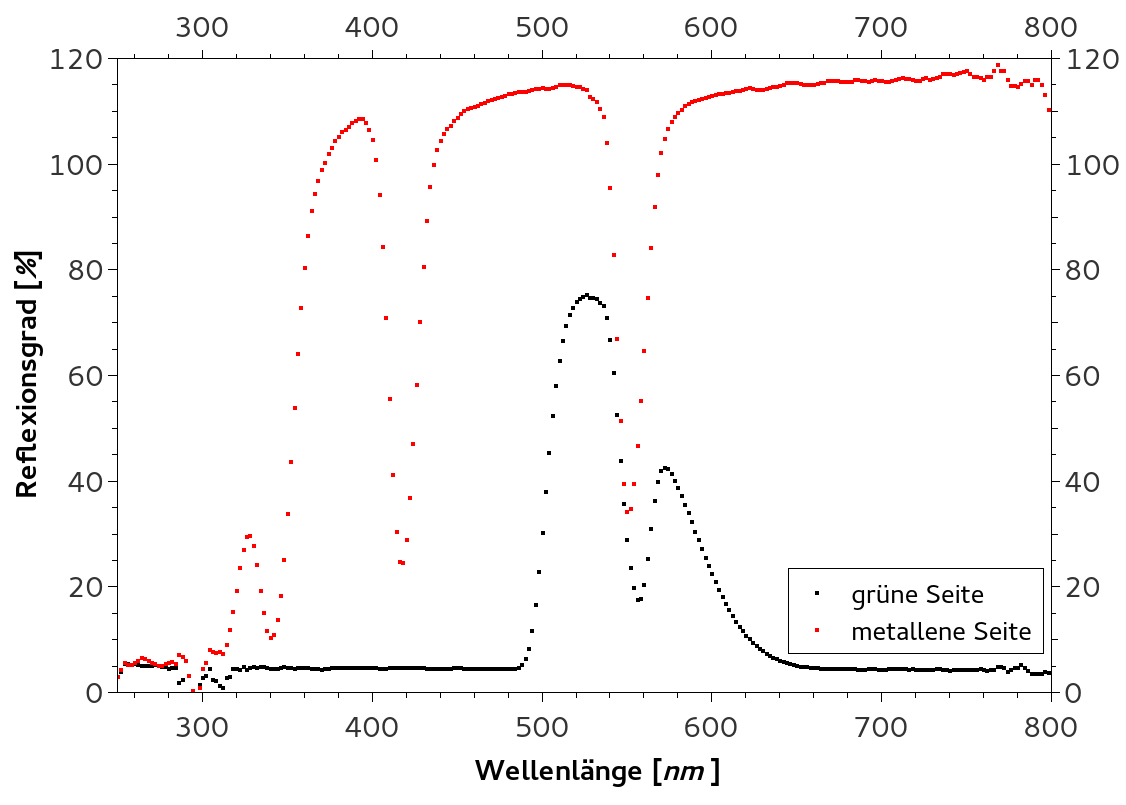
\includegraphics[scale=.22]{pic/RmetIntFilt.png}}
            \caption{Transmissions- und Relfexionsgrade eines Metall-Interferenz-Filters}
            \label{exp:MetInt}
        \end{figure}
        Abbildung \ref{exp:TMetInt} zeigt die Transmission in Abhängigkeit des Winkels. Dabei bedeutet \textit{gerade} den rechtwinkligen Einfall des Lichtes, \textit{gedreht} bedeutet eine Drehung um ca. $40\unit{°}$ und \textit{schief} bzw. \textit{schiefer} bedeuten eine Drehung von ungefähr $60\unit{°}$. Abbildung \ref{exp:TMetInt} zeigt eine Abhängigkeit der Wellenlänge des transmittierten Lichtes vom Einfallswinkel. Alle anderen Komponenten des Lichts werden entweder absorbiert oder reflektiert. Diese Beobachtung ist wiederum mit der Bragg-Bedingung erklärbar. Durch die Bedampfung des Trägers mit einer Metallschicht, ergibt sich ein Kristallgitter, für welches die Gleichungen \ref{bragg1} bzw. \ref{eq:gitter} gelten. Ändert man nun den Einfallswinkel unter Konstanz der Ordnung, ändert sich entsprechend die Wellenlänge des transmittierten Lichtes.
        Ein ähnlicher Gedanke erklärt auch die Kurve des Reflexionsgrades der metallenen Seite. Man kann deutlich wiederkehrende Minima erkennen, deren Abstände sich nahezu verdoppeln. Aus der Bragg-Bedingung könnte sich damit das nächste Minimum bei $840\unit{nm}$ befinden.
        Die grüne Seite des Metall-Interferenz-Filters reflektiert erwartungsgemäß vor allem grünes Licht. Die beiden Peaks entsprechen \unit[525]{nm} und \unit[575]{nm}.
    \subsubsection{Material des Visieres eines Feuerwehrhelms}
        Weiterhin wurde das Material, aus dem das Visier eines Feuerwehrhelms besteht, untersucht. Die Probe hat beschichtete und unbeschichtete Stellen. Transmissions- und Reflexionsgrade sind in Abbildung \ref{exp:feuerwehr} dargestellt.
        \begin{figure}[htbp]
            \subfigure[Transmission der beschichteten und unbeschichteten Seiten\label{exp:Tfeuer}]{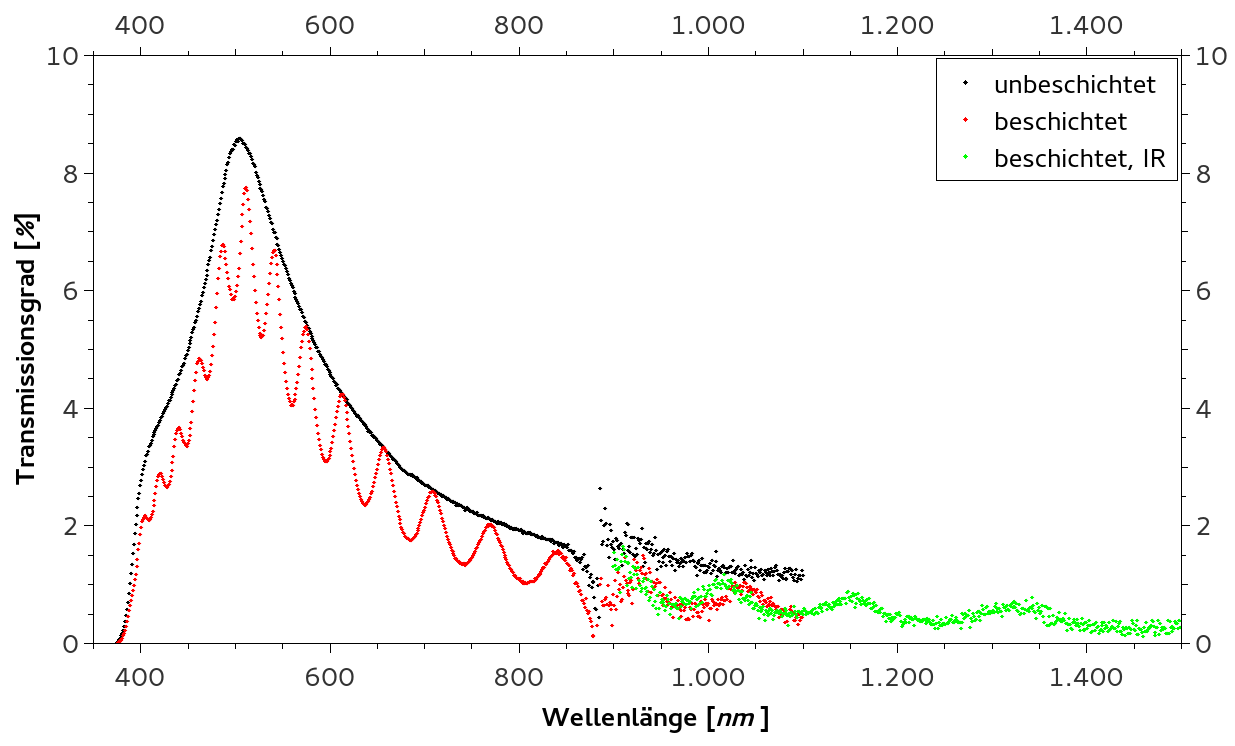
\includegraphics[scale=.2]{pic/TFeuerwehr.png}}
            \subfigure[Reflexion an beschichtetem und unbeschichtetem Visierelement\label{exp:Rfeuer}]{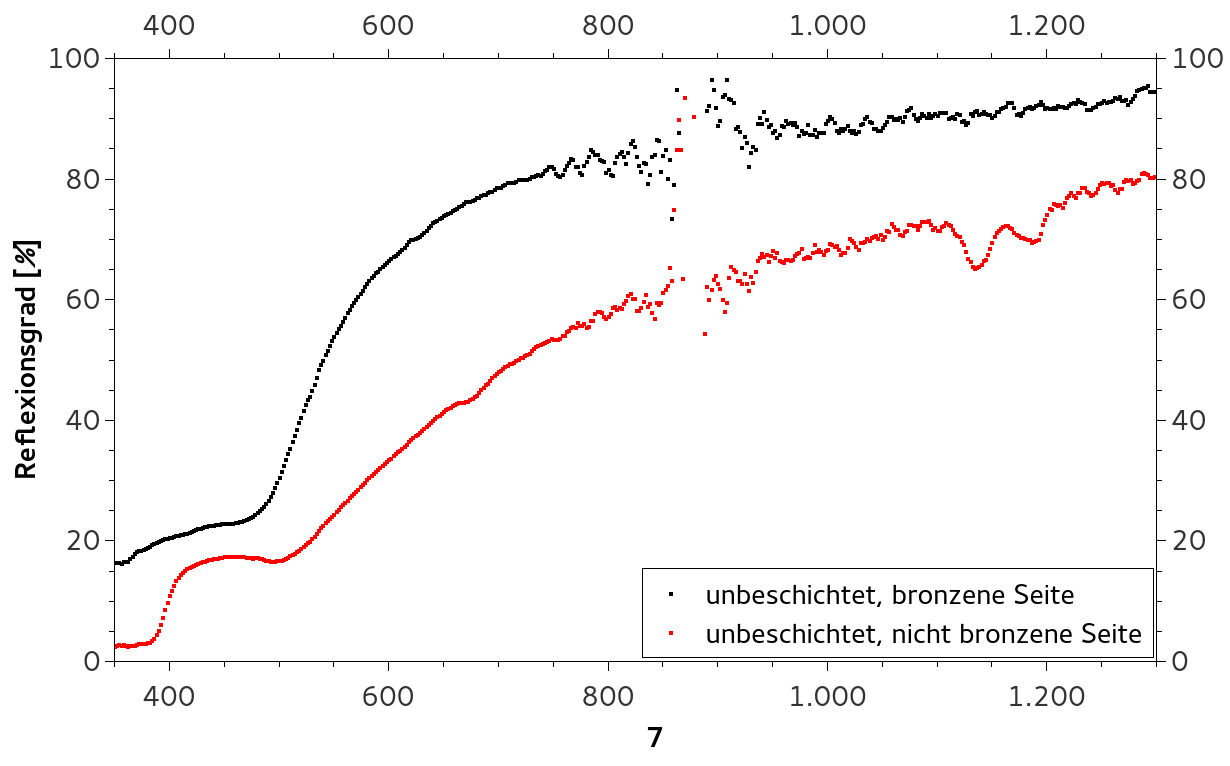
\includegraphics[scale=.2]{pic/RFhelmUnbesch.png}}
            \caption{Transmissions- und Relfexionsspektren eines Feuerwehrhelm-Visiers}
            \label{exp:feuerwehr}
        \end{figure}
        Abbildung \ref{exp:Tfeuer} zeigt drei Messungen. Die \textit{grüne} Linie ist schlicht die Fortsetzung der \textit{Roten} im Infrarotbereich, wobei man am Übergang erkennen kann, dass die Probe etwas verschoben wurde. Die Messung zeigt ein fluktuierendes Muster, welches als eine Art Umhüllende die Kurve der unbeschichteten Seite hat.
        Um diese Fluktuation zu erklären, kann ebenfalls Gleichung \ref{bragg1} herangezogen werden. Damit sind die Fluktuationen ein Muster konstruktiver Interferenz. Insgesamt lassen die unbeschichtete und die beschichtete Seite wenig Licht transmittieren
        In Abbildung \ref{exp:Rfeuer} ist die Reflexionsmessung an der unbeschichteten Seite zu sehen. Hieraus kann man im Zusammenhang mit Abb. \ref{exp:Tfeuer} erkennen, dass im Bereich zwischen \unit[350]{nm} und \unit[550]{nm} das meiste Licht absorbiert wird. Danach wird der weitaus größte Anteil von Licht reflektiert. Letzteres ist insbesondere bei hohen Temperaturen erwünscht, damit der Träger des Visiers im Einsatz entsprechend geschützt ist und sich der Helm nicht erhitzt. In \ref{exp:Rfeuer} kann man auch nochmal das Umschalten zwischen den Lampen beobachten. Um \unit[885]{nm} fluktuieren die Messwerte enorm. Ansonsten zeigt die unbeschichtete, nicht bronzene Seite ein schlechteres Reflexionsverhalten als die bronzene.
	\subsubsection{Farbstoffaufdampfschicht} \label{sec:organisch}
		Es wurde eine Glasplatte untersucht, auf die eine dünne Schicht eines lumineszierenden organischen Stoffgemisches aufgedampft wurde. Diese Schicht besteht zu 2\% aus Dichlormethan (DCM), einer organischen Substanz, die man häufig als Lösungsmittel für Harze, Fette und Kunststoffe verwendet\cite{dcm}, und zu 18 \% aus Aluminium-tris(8-hydroxychinolin) (Alq3), einer orange fluoreszierenden Komplexverbindung, welche zum Bau von organischen Leuchtdioden (OLED) verwendet wird.  Abbildung \ref{fig:TRA_organisch} zeigt das spektrale Verhalten der Messung in Transmission und Reflexion, sowie das Absorptionsverhalten. Man erkennt, dass die Absorption für Licht im UV-Bereich stark zunimmt, was dem typischen Verhalten einer Glasplatte, auf die das Substrat aufgebracht ist, entspricht (vergleiche Abbildung \ref{fig:R_T_glas}). Man erkennt mehrere Peaks zum einen im Bereich von etwa $\unit[400]{nm}$, welche mit dem Absorptionsverhalten von Alq3 erklärt werden können und in der Umgebung von etwa \unit[500]{nm}, die dem DCM zugeordnet werden können.\\
		\begin{figure}[htb]
			\centering
			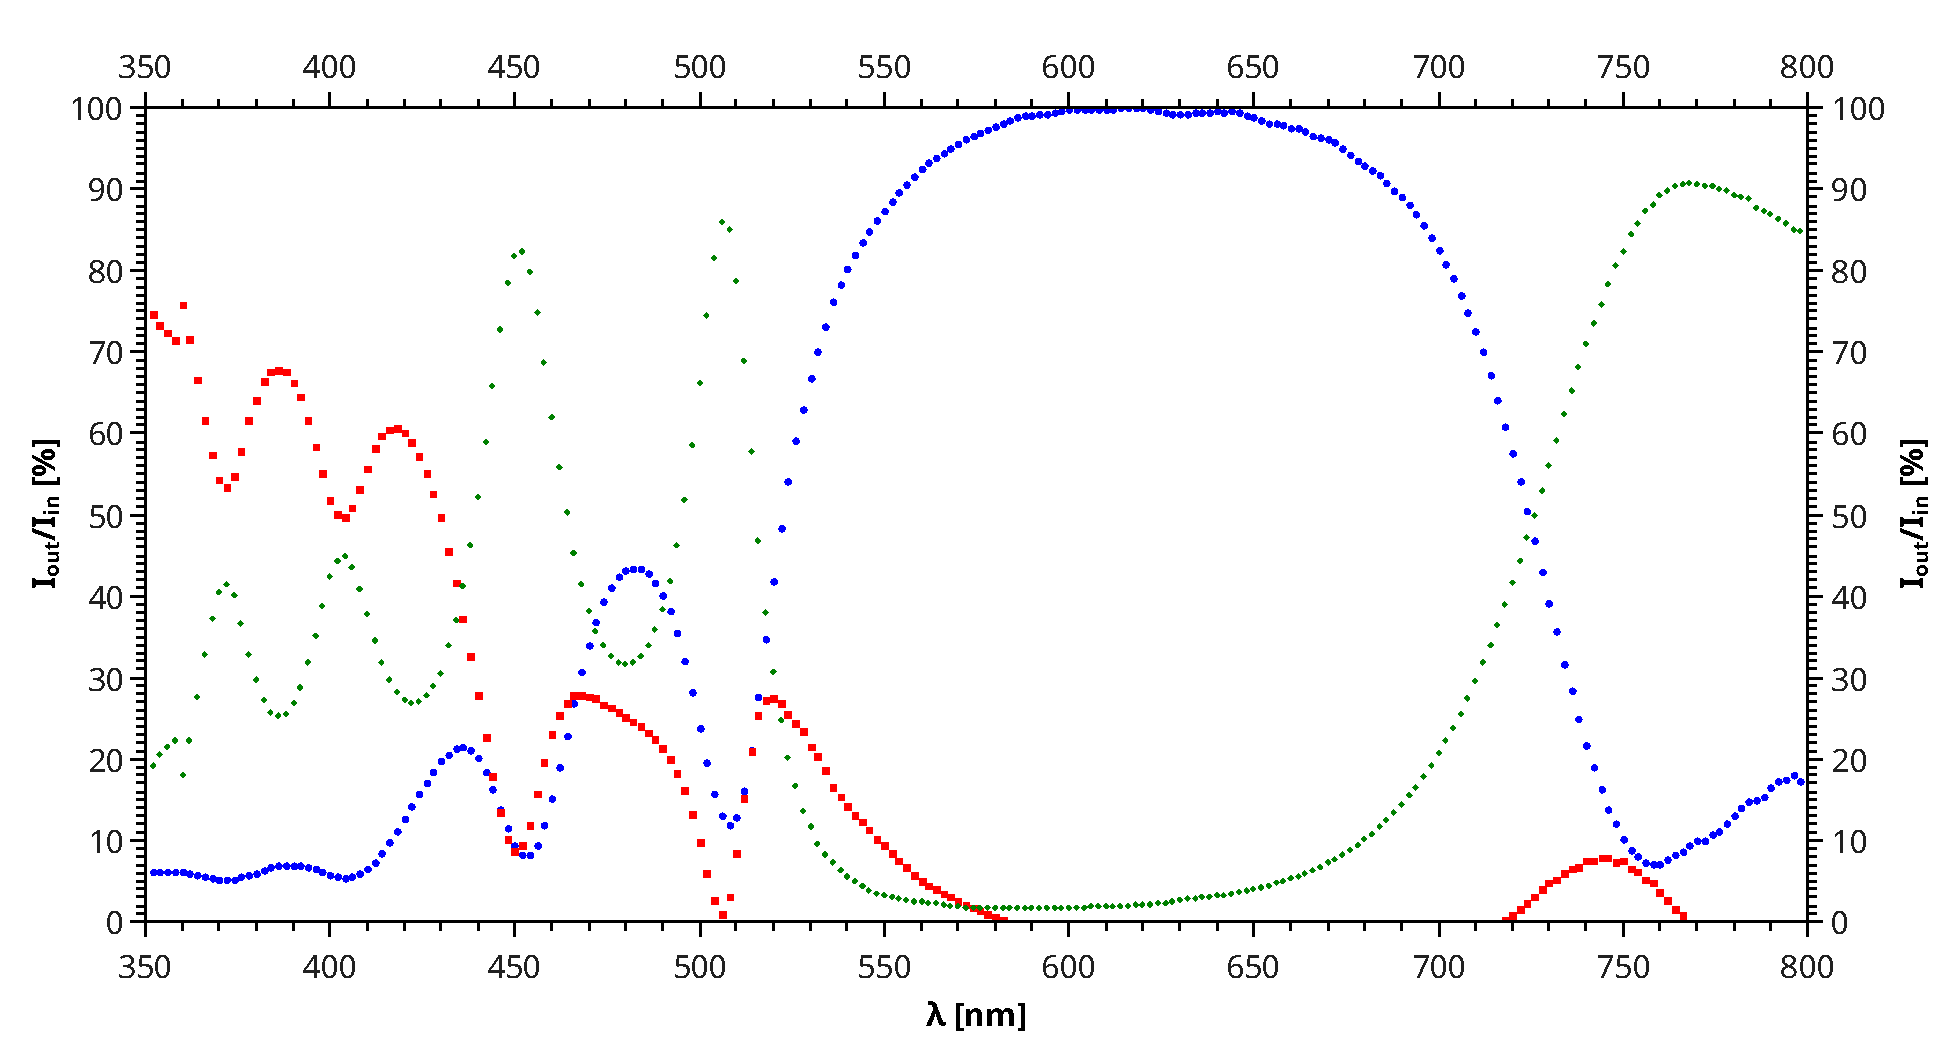
\includegraphics[width=0.75\linewidth]{pic/TRA_organisch.pdf}
			\caption{Spektrales Transmissions- (grün), Reflexions- (blau) und Absorptionsvermögen (rot) der Farbstoffaufdampfschicht. Aufgetragen ist das Verhältnis der Intensität des Probestrahles $I_{out}$ zu der des Referenzstrahles $I_{in}$ in Abhänigkeit der Wellenlänge des Strahles $\lambda$.}
			\label{fig:TRA_organisch}
		\end{figure} 
		Das Fluoreszenzverhalten dieser Probe wurde mit der in Abschnitt \ref{sec:fluoromax} beschriebenen Messmethode weiter untersucht. Dafür wurde die Probe mit 280, 400 und \unit[500]{nm} angeregt und es wurde die spektrale Intensität des emittierten Fluoreszenzlichtes gemessen. Diese speziellen Wellenlängen wurden gewählt, da bei diesen besonders starke Absorption zu erwarten ist. Abbildung \ref{fig:flouromax_emission} veranschaulicht die Ergebnisse der Messung.
		\begin{figure}[htb]
			\centering
			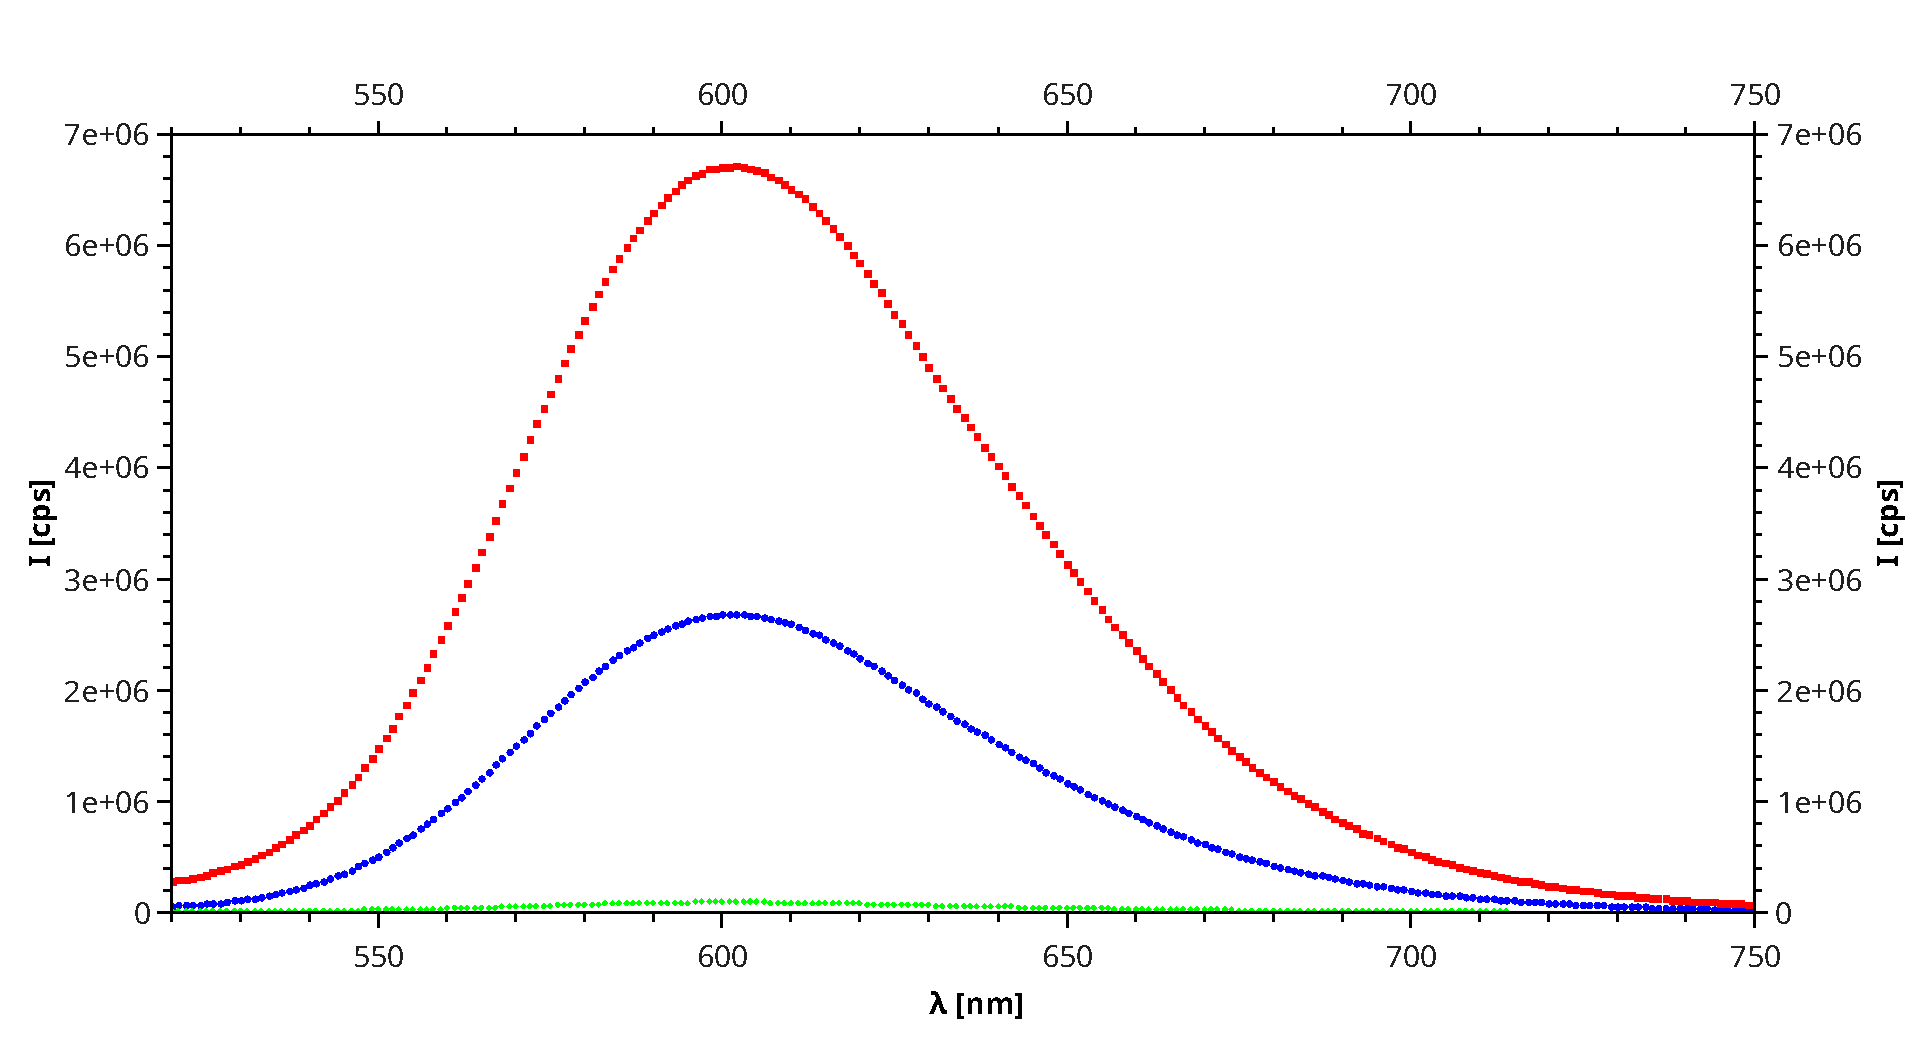
\includegraphics[width=0.75\linewidth]{pic/flouromax_emission.pdf}
			\caption{Emissionsspektrum der Farbaufdampfschicht unter Bestrahlung mit \unit[280]{nm} (grün), \unit[400]{nm} (rot), \unit[500]{nm} (blau). Dargestellt ist die emittierte Intensität des Fluoreszenzlichtes $I$ in Einheiten der Detektorzählimpulse pro Zeitheiten als Funktion der Wellenlänge $\lambda$.}
			\label{fig:flouromax_emission}
		\end{figure}
		Man sieht deutlich, dass in allen drei Fällen ein Intensitätspeak bei \unit[600]{nm} entsteht, welcher das orangefarbene Fluoreszenzlicht erklärt. Das offensichtlich größte Maximum entsteht, wenn man direkt mit \unit[400]{nm} die Alq3-Moleküle in einen höheren Anregungszustand versetzt, welche bei Abregung dann Photonen der entsprechenden Wellenlänge emittieren. Mit \unit[280]{nm} regt man hauptsächlich das Glasgitter an. Dieses gibt die Anregung zum Beispiel in Form von Gitterschwingungen (Phononen) an Alq3 weiter, welches dann fluoresziert. Der resultierende Peak ist allerdings sehr klein im Vergleich zur direkten Anregung. Bei \unit[500]{nm} wird Dichlormethan besonders häufig angeregt. Auf organische Moleküle wie DCM wirkt sich eine Anregung auf den Schwinguns- und Rotationszustand aus, wodurch auch hier Energie an Alq3 weitergegeben werden kann. 